\documentclass{beamer}

\usepackage[utf8]{inputenc} % Set Encoding
\usepackage[T1]{fontenc} % Enable cyrillic fonts
\usepackage{fontspec} % Using custom fonts (requires -xelatex flag)
\usepackage{graphicx} % For image insertions
\usepackage{float} % For positioning
\usepackage[section]{placeins}
\usepackage{fontspec}
\usepackage{minted} % For code listing

\setmainfont[
  Ligatures=TeX,
  Extension=.otf,
  BoldFont=cmunbx,
  ItalicFont=cmunti,
  BoldItalicFont=cmunbi,
]{cmunrm}
\setsansfont[
  Ligatures=TeX,
  Extension=.otf,
  BoldFont=cmunsx,
  ItalicFont=cmunsi,
]{cmunss}

\setbeamertemplate{footline}[frame number]
\beamertemplatenavigationsymbolsempty
\setlength{\parskip}{1em}

\title{Бот Dvango}
\subtitle{Системи інтелектуальної обробки природо-мовної інформації}
\author[Апраксін, Соколенко]{
    Апраксін Антон Романович
    \and\\
    Соколенко Дмитро Олександрович
}
\institute[ХНУРЕ]{ІТШІ-18-1}
\date{Харків 2021}

\begin{document}
\frame{\titlepage}

\begin{frame}
    \frametitle{Вступ}

    Дана робота присвячена побудові чатботу, що відповідає на запитання користувача.
    % цель нашей работы это построить чатбот, который отвечает на вопросы пользователя в форме естественного языка

    \begin{itemize}
        \item Не може підтримувати діалог.
        % вслух
        % наш бот не может поддерживать диалог на бытовые темы, поэтому ему нельзя написать "привет" или "как дела?" так как это не является его целью


        \item Дуже гарно відповідає на запитання.
        % вслух
        % Но бот очень хорошо (как для бота) отвечает на вопросы, которые поставил пользователь.
        \item Використовує нейронні мережі.
        % вслух
        % и для нахождения ответа он использует нейронные сети
    \end{itemize}
    
\end{frame}

\begin{frame}
    \frametitle{Актуальність}
    Ми живемо в епоху інформаційних технологій, які увійшли у життя кожного з нас. 
    % мы живём в эпоху информационных технологий, которые стали частью жизни каждого из нас

    Бізнеси з онлайн присутністю повсюдно впроваджують чат-ботів для відповідання на питання клієнтів.
    % бизнесы с онлайн присутствием повсеместно вводят в использование чат-ботов для ответа на всевозможные вопросы клиентов
    % и чтобы оставаться конкурентноспособными компаниям нужно вводить новых чат-ботов и модернизировать существующих

    % с другой стороны технологии машинного обучения тоже развиваются.
    Технології машинного навчання за останні роки значно просунулися.
    % вслух
    % можно вспомнить GPT-3, который создаёт очень правдоподобные тексты, и их не всегда можно отличить от написанных человеком

    % и это приводит нас к мысли: использовать современные технологии для решения современных проблем

    Ми можемо побудувати систему, яка буде знаходити відповіді на питання з різних тем. І робити система це може інтерактивно, у вигляді чат-боту, якому ви пишете повідомлення, яке містить питання і на яке бот якось змістовно відповідає.
    % То есть мы можем построить такую систему, что будет знаходити ОТВЕТЫ на вопросы, что нас интересуют. И делать система это может интерактивно, то есть в формате чатбота, которому вы пишете сообщение, и на которое бот даёт содержательный ответ

\end{frame}

\begin{frame}
    \frametitle{Історія розвитку}
    % люди задумлись о создании систем обработки естественного языка с того к появились первые компьютеры
    \begin{itemize}
        \item ELIZA.
        В її основі лежить алгоритм, що перефразовував питання користувача, виділяючи в ньому незмінну частину.
        % Одним з перших віртуальних чатботів була програма ELIZA. В її основі лежить алгоритм, що перефразовував питання користувача, виділяючи в ньому незмінну частину. Однако бота можно было раскрыть всего за два вопроса.

        \item PARRY.
        Симулював людину хвору на шизофренію.
        % в эксперименте он смог обмануть группу экспертов, и его не смогли отличить от других пациентов
    \end{itemize}
    % Затем появлялись более современные и продвинутые модели. С появлением нейронных сетей мощность таких систем сильно возросла. Начали появляться системы, которые могут ввести в заблуждение более 50% жюри.

    Сьогодні віртуальних асистентів можна зустріти у більшості компаній. Вони допомагають користувачам вирішувати проблеми, що виникають при користуванні системою.
    % Сегодня виртуальных ассистентов можно встретить в большинстве компаний. Они помогают пользователям решать проблемы, возникающие при пользовании системой.
\end{frame}

\begin{frame}
    \frametitle{Відомі проекти}

    % из существующих проектов по этому направлению одни из самых известные это:
    \begin{enumerate}
        \item ELIZA -- перший більш-менш успішний проект
        \item PARRY -- з'явився трохи пізніше ELIZA. Пародував параноїдального шизофреніка.
        \item CleverBot -- пройшов 59\% тестів Тьюринга в 2011 році.
    \end{enumerate}

    % и ещё множество других
    % большинство из них использует простые методы сопоставления с образцом и поиска по ключевым словам
    % а более современные подходы включают нейронные сети
\end{frame}

\begin{frame}
    \frametitle{Основні підходи до вирішення проблеми}
    Сьогодні існує багато алгоритмів, які допомагають будувати розумні системи з обробки природо-мовної інформації. Це і системи побудовані на простих алгоритмах, таких як наївний Байес або програма ELIZA.
    % Сегодня существует много алгоритмов, которые помогают строить умные системы по обработке природно-языковой информации. Это и системы построенные на простых алгоритмах, как наивный Байес или программа ELIZA.

    Але також існують нейронні мережі, в яких набагато більний потенціал. Архітектура сучаної нейромережі, що часто використовується -- трансформер. Саме цю архітектуру ми використовували.
    % с увеличением вычислительных мощностей нейронные сети стали более актуальными, и на данный момент решают задачи работы с естесственным языком наиболее хорошо
    % на данный момент самой лучшей архитектурой нейронной сети является трансформер, которую мы и использовали в данной работе
\end{frame}

\begin{frame}
    \frametitle{Архітектура бота}
    Програма представляє собою Telegram чат-бота, який відповідає на запитання користувача. Теми запитань мають бути заздалегідь описані в базі даних чат-бота. Як основний компонент роботи інтелекту бота використовується нейронна мережа BERT-large, заздалегідь натренована на датасеті SQuAD. Як допоміжний використовується алгоритм FlashText.
\end{frame}

\begin{frame}
    \frametitle{Організація бази даних}
    \inputminted[breaklines,linenos=true]{yaml}{sample.yaml}
\end{frame}

\begin{frame}
    \frametitle{Архітектура трансформерів}
    \begin{figure}[H]
        \centering
        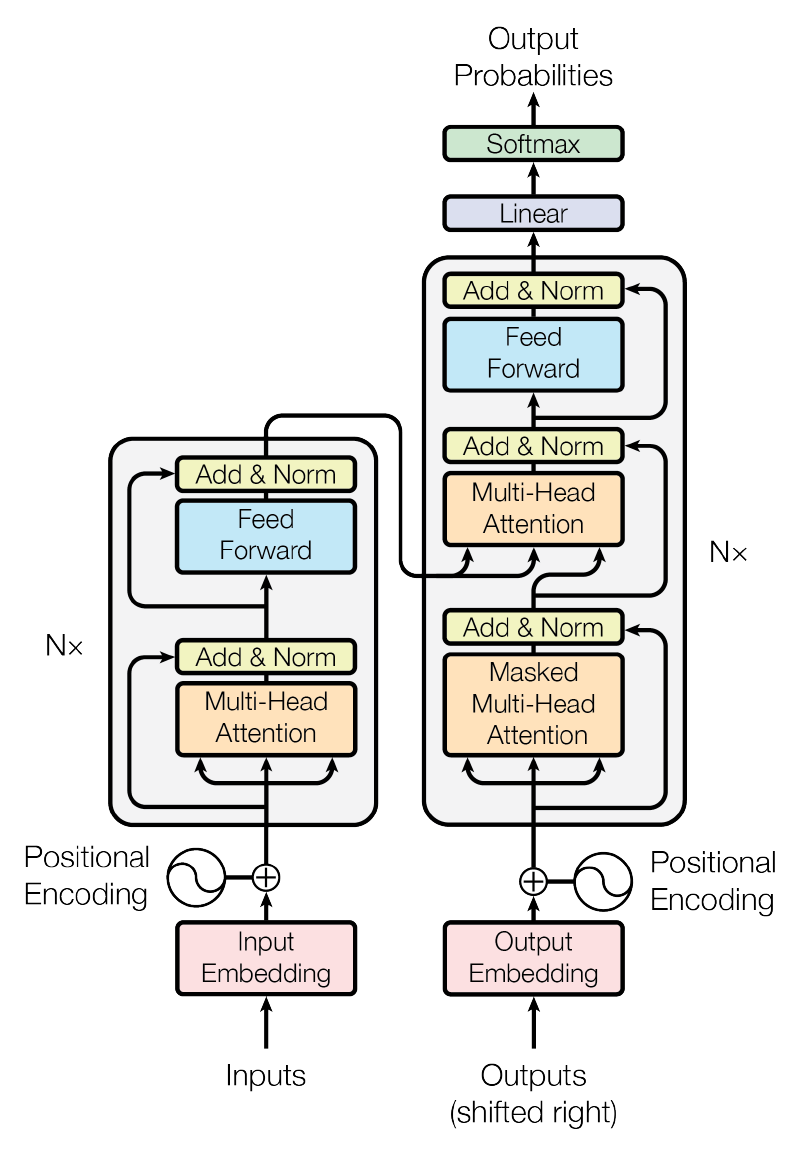
\includegraphics[width=0.5\textwidth]{transformer.png}
    \end{figure}
\end{frame}

\begin{frame}
    \frametitle{Шар уваги}
    \begin{figure}[H]
        \centering
        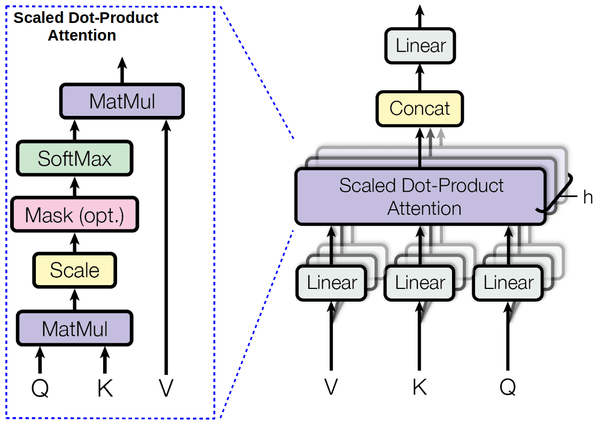
\includegraphics[width=0.6\textwidth]{attention_layer.png}
    \end{figure}
\end{frame}

\begin{frame}
    \frametitle{Перспективи розвитку}
    Вирішити проблеми:

    \begin{itemize}
        \item бот повільний;
        \item при великому розмірі контексту конкретної теми довго відповідає;
        \item вибір теми по ключовим словам не обробляє деякі випадки.
    \end{itemize}

    Можливі рішення:
    
    \begin{itemize}
        \item використати іншу модель для пошуку відповіді;
        \item на деяких етапах пошуку необхідного контексту використовувати додаткові алгоритми;
        \item покращити пошук за ключовими словами.
    \end{itemize}
\end{frame}

\begin{frame}
    \frametitle{Висновки}

    \begin{itemize}
        \item У процесі виконання роботи ми розробили бота, який відповідає на запитання користувача.
        \item Галузь розвивається дуже швидко, тому треба підтримувати актуальність своїх знань.
    \end{itemize}

    % вслух
    % Есть как академический так и коммерческий интерес. Ученые хотят первыми пройти успешно тест Тьринга, компании пытаются как можно больше все автоматизировать, поэтому тоже инвестируют в эту отрасль. Мы должны поддерживать уровень актуальности своих знаний.
\end{frame}

\end{document}
